{
\renewcommand{\thechapter}{\arabic{chapter}R}
\setcounter{chapter}{15}
\exam{Exam resource 2015/16}

\question{Question 1}
Mr Silva has 1000\euro that he wants to invest in BLA shares. He guarantees he known the values those stocks will have in the following $n$ days. Mr Silva wants to choose one (and only one) day to buy as many stocks as possible and another day, afterwardsm to sell all actions. The point is to maximize profit. Consider \texttt{price[]} to be the vector containing the prices of BLA shares in the following days, where \texttt{price[i]} is the price of a stock in day $i$.

\questionitem{Item a}
Implement in pseudocode a solution to this problem, using a divide-and-conquer strategy. Explain and mention its time complexity.

\ansseparator

Our function $solve(l,r)$ returns the best day to buy (minimum price) and best day to sell (maximum price) enforcing the condition that the best day to sell is after the best day to buy, and both days are in $[l,r)$.

We will assume one can buy and sell stock in the same day, so we can account for a strictly decreasing $price$.

The base case is $solve(i, i+1)=(i,i)$, because in a 1-day interval the best day to buy and sell is that one available day.

The recursivity that allows us to develop a divide-and-conquer approach is that, for $solve(l,r)$, we can run $solve$ for the left and right halves, and then merge those results using the best of the three possible solutions:
\begin{enumerate*}
    \item Buy and sell in the left half;
    \item Buy and sell in the right half;
    \item Buy in the left half and sell in the right half.
\end{enumerate*}

\begin{algorithm}[H]
    \caption{2016R-01a}
    \begin{algorithmic}[1]
        \Function{solve}{$price$, $l$, $r$}
            \If{$r-l = 1$}{ \Return{$(l, l)$}}
            \EndIf
            \State{$m \gets (l+r)/2$}
            \State{$(b_1, s_1) \gets \Call{solve}{price, l, m}$}
            \State{$(b_2, s_2) \gets \Call{solve}{price, m, r}$}
            \State{$(b,s) \gets (l,l)$}
            \If{$price[s] - price[b] < price[s_1] - price[b_1]$}{ $(b, s) \gets (b_1, s_1)$}
            \EndIf
            \If{$price[s] - price[b] < price[s_2] - price[b_2]$}{ $(b, s) \gets (b_2, s_2)$}
            \EndIf
            \If{$price[s] - price[b] < price[s_2] - price[b_1]$}{ $(b, s) \gets (b_1, s_2)$}
            \EndIf
            \State \Return $(b, s)$
        \EndFunction
    \end{algorithmic}
\end{algorithm}

\newpage
Our recurrence is reflected in terms of complexity as

\begin{equation*}
    T(n) = 2T(n/2) + 1 \iff \begin{cases}
        T(n) = a\,T(n/b) + f(n) \\
        a = 2 \\
        b = 2 \\
        f(n) = O(1)
    \end{cases}
\end{equation*}

where $T(n)$ is the time it takes to run $solve(l, r)$ with $n = r-l$.

\begin{theorem}[Master theorem for divide-and-conquer recurrences]
    Let $a, b \geq 1$ be constants, left $f(n)$ be a function and left $T(n)$ be defined on the nonnegative integers by the recurrence
    \begin{equation*}
        T(n) = a\,T(n/b) + f(n)
    \end{equation*}
    (where $n/b$ is interpreted as either $\lfloor n/b \rfloor$ or $\lceil n/b \rceil$). Then $T(n)$ has the following asymptotic bounds:
    \begin{enumerate}
        \item $f(n) = O(n^{\log_b{a} - \varepsilon})$ for some constant $\varepsilon > 0$ $\implies T(n) = \Theta(n^{\log_b{a}})$
        \item $f(n) = \Theta(n^{\log_b{a}}) \implies T(n) = \Theta(n^{\log_b{a}} \log{n})$
        \item $f(n) = O(n^{\log_b{a} + \varepsilon})$ for some constant $\varepsilon > 0$, and $a f(n/b) \leq c f(n)$ for some constant $c < 1$ and $n$ asymptotically large $\implies T(n) = \Theta(f(n))$
    \end{enumerate}
\end{theorem}


We know $\log_b{a} = \log_2{2} = 1$. Since $f(n) = O(1) = O(n^0) = O(n^{1-1}) = O(n^{\log_b{a}-\varepsilon})$ where $\varepsilon = 1$ is a positive constant, we know by the master theorem that $T(n) \in \Theta (n^{\log_b{a}})$; $\Theta (n^{\log_b{a}}) = \Theta (n^1) = \Theta(n) \subseteq O(n)$, so $T(n) \in O(n)$ meaning this algorithm takes time linear in $n$.

\questionitem{Item b}
We now want to solve the problem using dynamic programming. Formalize a solution to this problem, presenting its recurrence formula. Implement that solution in pseudocode. Explain and mention its time complexity.

\ansseparator

$buy(i)$ is the best day to buy in $[0,i]$. $sell(i)$ is the best day to sell in $[i,n)$. $S_i$ is the solution if you decide to buy before or at day $i$ and sell after or at day $i$.

\begin{alignat*}{2}
    S_i     &= sell(i) - buy(i) \\
    buy(i)  &= \begin{dcases}
        0                          &: i=0 \\
        buy(i-1) &: price(i) \geq price(buy(i-1)) \\
        i        &: price(i) <    price(buy(i-1))
    \end{dcases} \\
    sell(i) &= \begin{dcases}
        n-1                         &: i=n-1 \\
        sell(i+1) &: price(i) <    price(sell(i+1)) \\
        i         &: price(i) \geq price(sell(i+1))
    \end{dcases}
\end{alignat*}

This solution takes time $O(n)$ since it takes $O(n)$ to calculate $buy$ and $sell$, and the last cycle iterates over $n$ elements.

\newpage
\begin{algorithm}[H]
    \caption{2016R-01b}
    \begin{algorithmic}[1]
        \Function{solve}{$price$, $n$}
            \State {$buy(0) \gets 0$}
            \For{$i \gets 1:n-1$}
                \If{$price(i) \geq price(buy(i-1))$}{ $buy(i) \gets buy(i-1)$}
                \Else { $buy(i) \gets i$}
                \EndIf
            \EndFor
            \State {$sell(n-1) \gets n-1$}
            \For{$i \gets n-2:0$}
                \If{$price(i) < price(sell(i-1))$}{ $sell(i) \gets sell(i+1)$}
                \Else { $sell(i) \gets i$}
                \EndIf
            \EndFor
            \State{$(b, s) \gets (buy(0), sell(0))$}
            \For{$i \gets 1:n-1$}
                \If{$price(s)-price(b) < price(sell(i)) - price(buy(i))$}
                    \State {$(b, s) \gets (buy(i), sell(i))$}
                \EndIf
            \EndFor
            \State \Return $(b, s)$
        \EndFunction
    \end{algorithmic}
\end{algorithm}

\question{Question 2}
The following graph represents a road map. Vertices correspond to cities, and edges' values to the distance between cities.

\begin{center}
    \begin{tikzpicture}[->,>=stealth',node distance=2cm,initial text=$ $,]
		\node[state](A) {$A$};
        \node[state, above right of=A](B) {$B$};
        \node[state, below right of=A](D) {$D$};
        \node[state, right of=B](C) {$C$};
        \node[state, right of=D](E) {$E$};
        \node[state, below right of=C](F) {$F$};
        
        \draw   (A) 	edge[above] node{7} (B)
                (A) 	edge[below] node{2} (D)
                (B) 	edge[above] node{2} (C)
                (C) 	edge[left ] node{4} (E)
                (C) 	edge[above] node{5} (F)
                (D) 	edge[left ] node{3} (B)
                (D) 	edge[above] node{8} (C)
                (D) 	edge[below] node{4} (E)
                (E) 	edge[below] node{8} (F)
                ;
	\end{tikzpicture}
\end{center}

\questionitem{Item a}
Using Dijkstra's algorithm, find the shortest path from city $A$ to city $F$. Show all intermediate steps, explaining.

\ansseparator

\begin{algorithm}[H]
    \caption{Dijkstra's algorithm}
    \begin{algorithmic}[1]
        \Function{Dijkstra}{$G(V,E,w)$, $s$}
            \For{$v \in V$}{ $dist(v) \gets \infty,~prev(v) \gets \text{NULL}$}
            \EndFor
            \State {$Q \gets V$}
            \State {$dist(s) \gets 0$}
            \While{$|Q| > 0$}
                \State {$u \gets \text{vertex of $Q$ with least $dist(u)$}$}
                \State {$Q \gets Q \backslash \{u\}$}
                \For{$v \in \Call{Adj}{G, u}$}
                    \State{$c' \gets dist(u) + w(u,v)$}
                    \If{$c' < dist(v)$}
                        \State{$dist(v) \gets c',~prev(v) \gets u$}
                    \EndIf
                \EndFor
            \EndWhile
            \State \Return $dist$, $prev$
        \EndFunction
    \end{algorithmic}
\end{algorithm}

Above each node is the distance and previous node in the shortest path.

Nodes in light gray are visited, node in dark gray is active (current value of $u$). Nodes in light and dark gray are not in $Q$.

\begin{center}
    \begin{longtable}{P{76mm} | P{76mm}}
        \textbf{Line 5} & \textbf{Line 8} \\ \hline 
        \begin{tikzpicture}[->,>=stealth',node distance=2cm,initial text=$ $,]
            \node[state                  , label=above:{$     0, -$}](A) {$A$};
            \node[state, above right of=A, label=above:{$\infty, -$}](B) {$B$};
            \node[state, below right of=A, label=below:{$\infty, -$}](D) {$D$};
            \node[state, right of=B      , label=above:{$\infty, -$}](C) {$C$};
            \node[state, right of=D      , label=below:{$\infty, -$}](E) {$E$};
            \node[state, below right of=C, label=above:{$\infty, -$}](F) {$F$};
            
            \draw   (A) 	edge[above] node{7} (B)
                    (A) 	edge[below] node{2} (D)
                    (B) 	edge[above] node{2} (C)
                    (C) 	edge[left ] node{4} (E)
                    (C) 	edge[above] node{5} (F)
                    (D) 	edge[left ] node{3} (B)
                    (D) 	edge[above] node{8} (C)
                    (D) 	edge[below] node{4} (E)
                    (E) 	edge[below] node{8} (F)
                    ;
        \end{tikzpicture} &
        \begin{tikzpicture}[->,>=stealth',node distance=2cm,initial text=$ $,]
            \node[state                  , label=above:{$     0, -$}, fill=activecolor ](A) {$A$};
            \node[state, above right of=A, label=above:{$\infty, -$}](B) {$B$};
            \node[state, below right of=A, label=below:{$\infty, -$}](D) {$D$};
            \node[state, right of=B      , label=above:{$\infty, -$}](C) {$C$};
            \node[state, right of=D      , label=below:{$\infty, -$}](E) {$E$};
            \node[state, below right of=C, label=above:{$\infty, -$}](F) {$F$};
            
            \draw   (A) 	edge[above] node{7} (B)
                    (A) 	edge[below] node{2} (D)
                    (B) 	edge[above] node{2} (C)
                    (C) 	edge[left ] node{4} (E)
                    (C) 	edge[above] node{5} (F)
                    (D) 	edge[left ] node{3} (B)
                    (D) 	edge[above] node{8} (C)
                    (D) 	edge[below] node{4} (E)
                    (E) 	edge[below] node{8} (F)
                    ;
        \end{tikzpicture} \\
        We start by setting $dist(A) \gets 0$. &
        Select node in $Q$ with least $dist$, which is $A$. \\ \\
        \begin{tikzpicture}[->,>=stealth',node distance=2cm,initial text=$ $,]
            \node[state                  , label=above:{$     0, -$}, fill=visitedcolor ](A) {$A$};
            \node[state, above right of=A, label=above:{$     7, A$}, double](B) {$B$};
            \node[state, below right of=A, label=below:{$     2, A$}, double](D) {$D$};
            \node[state, right of=B      , label=above:{$\infty, -$}](C) {$C$};
            \node[state, right of=D      , label=below:{$\infty, -$}](E) {$E$};
            \node[state, below right of=C, label=above:{$\infty, -$}](F) {$F$};
            
            \draw   (A) 	edge[above] node{7} (B)
                    (A) 	edge[below] node{2} (D)
                    (B) 	edge[above] node{2} (C)
                    (C) 	edge[left ] node{4} (E)
                    (C) 	edge[above] node{5} (F)
                    (D) 	edge[left ] node{3} (B)
                    (D) 	edge[above] node{8} (C)
                    (D) 	edge[below] node{4} (E)
                    (E) 	edge[below] node{8} (F)
                    ;
        \end{tikzpicture} &
        \begin{tikzpicture}[->,>=stealth',node distance=2cm,initial text=$ $,]
            \node[state                  , label=above:{$     0, -$}, fill=visitedcolor](A) {$A$};
            \node[state, above right of=A, label=above:{$     7, A$}](B) {$B$};
            \node[state, below right of=A, label=below:{$     2, A$}, fill=activecolor ](D) {$D$};
            \node[state, right of=B      , label=above:{$\infty, -$}](C) {$C$};
            \node[state, right of=D      , label=below:{$\infty, -$}](E) {$E$};
            \node[state, below right of=C, label=above:{$\infty, -$}](F) {$F$};
            
            \draw   (A) 	edge[above] node{7} (B)
                    (A) 	edge[below] node{2} (D)
                    (B) 	edge[above] node{2} (C)
                    (C) 	edge[left ] node{4} (E)
                    (C) 	edge[above] node{5} (F)
                    (D) 	edge[left ] node{3} (B)
                    (D) 	edge[above] node{8} (C)
                    (D) 	edge[below] node{4} (E)
                    (E) 	edge[below] node{8} (F)
                    ;
        \end{tikzpicture} \\
        \begin{minipage}[c]{1\linewidth}
            $B$ and $D$ are adjacent to $A$.\\
            $dist(A)+w(A,B) = 7 < \infty$ so $B$ was updated.\\
            $dist(A)+w(A,D) = 2 < \infty$ so $D$ was updated.
        \end{minipage} &
        Select node in $Q$ with least $dist$, which is $D$. \\ \\
        \begin{tikzpicture}[->,>=stealth',node distance=2cm,initial text=$ $,]
            \node[state                  , label=above:{$     0, -$}, fill=visitedcolor](A) {$A$};
            \node[state, above right of=A, label=above:{$     5, D$}, double](B) {$B$};
            \node[state, below right of=A, label=below:{$     2, A$}, fill=visitedcolor](D) {$D$};
            \node[state, right of=B      , label=above:{$    10, D$}, double](C) {$C$};
            \node[state, right of=D      , label=below:{$     6, D$}, double](E) {$E$};
            \node[state, below right of=C, label=above:{$\infty, -$}](F) {$F$};
            
            \draw   (A) 	edge[above] node{7} (B)
                    (A) 	edge[below] node{2} (D)
                    (B) 	edge[above] node{2} (C)
                    (C) 	edge[left ] node{4} (E)
                    (C) 	edge[above] node{5} (F)
                    (D) 	edge[left ] node{3} (B)
                    (D) 	edge[above] node{8} (C)
                    (D) 	edge[below] node{4} (E)
                    (E) 	edge[below] node{8} (F)
                    ;
        \end{tikzpicture} &
        \begin{tikzpicture}[->,>=stealth',node distance=2cm,initial text=$ $,]
            \node[state                  , label=above:{$     0, -$}, fill=visitedcolor](A) {$A$};
            \node[state, above right of=A, label=above:{$     5, D$}, fill=activecolor ](B) {$B$};
            \node[state, below right of=A, label=below:{$     2, A$}, fill=visitedcolor](D) {$D$};
            \node[state, right of=B      , label=above:{$    10, D$}](C) {$C$};
            \node[state, right of=D      , label=below:{$     6, D$}](E) {$E$};
            \node[state, below right of=C, label=above:{$\infty, -$}](F) {$F$};
            
            \draw   (A) 	edge[above] node{7} (B)
                    (A) 	edge[below] node{2} (D)
                    (B) 	edge[above] node{2} (C)
                    (C) 	edge[left ] node{4} (E)
                    (C) 	edge[above] node{5} (F)
                    (D) 	edge[left ] node{3} (B)
                    (D) 	edge[above] node{8} (C)
                    (D) 	edge[below] node{4} (E)
                    (E) 	edge[below] node{8} (F)
                    ;
        \end{tikzpicture} \\
        \begin{minipage}[c]{1\linewidth}
            $B$, $C$ and $E$ are adjacent to $D$.\\
            $dist(D)+w(D,B) = 5 < 7$ so $B$ was updated.\\
            $dist(D)+w(D,C) = 10 < \infty$ so $C$ was updated.\\
            $dist(D)+w(D,E) = 6 < \infty$ so $E$ was updated.
        \end{minipage} &
        Select node in $Q$ with least $dist$, which is $B$. \\ \\
        \begin{tikzpicture}[->,>=stealth',node distance=2cm,initial text=$ $,]
            \node[state                  , label=above:{$     0, -$}, fill=visitedcolor](A) {$A$};
            \node[state, above right of=A, label=above:{$     5, D$}, fill=visitedcolor](B) {$B$};
            \node[state, below right of=A, label=below:{$     2, A$}, fill=visitedcolor](D) {$D$};
            \node[state, right of=B      , label=above:{$     7, B$}, double](C) {$C$};
            \node[state, right of=D      , label=below:{$     6, D$}](E) {$E$};
            \node[state, below right of=C, label=above:{$\infty, -$}](F) {$F$};
            
            \draw   (A) 	edge[above] node{7} (B)
                    (A) 	edge[below] node{2} (D)
                    (B) 	edge[above] node{2} (C)
                    (C) 	edge[left ] node{4} (E)
                    (C) 	edge[above] node{5} (F)
                    (D) 	edge[left ] node{3} (B)
                    (D) 	edge[above] node{8} (C)
                    (D) 	edge[below] node{4} (E)
                    (E) 	edge[below] node{8} (F)
                    ;
        \end{tikzpicture} &
        \begin{tikzpicture}[->,>=stealth',node distance=2cm,initial text=$ $,]
            \node[state                  , label=above:{$     0, -$}, fill=visitedcolor](A) {$A$};
            \node[state, above right of=A, label=above:{$     5, D$}, fill=visitedcolor](B) {$B$};
            \node[state, below right of=A, label=below:{$     2, A$}, fill=visitedcolor](D) {$D$};
            \node[state, right of=B      , label=above:{$     7, B$}](C) {$C$};
            \node[state, right of=D      , label=below:{$     6, D$}, fill=activecolor ](E) {$E$};
            \node[state, below right of=C, label=above:{$\infty, -$}](F) {$F$};
            
            \draw   (A) 	edge[above] node{7} (B)
                    (A) 	edge[below] node{2} (D)
                    (B) 	edge[above] node{2} (C)
                    (C) 	edge[left ] node{4} (E)
                    (C) 	edge[above] node{5} (F)
                    (D) 	edge[left ] node{3} (B)
                    (D) 	edge[above] node{8} (C)
                    (D) 	edge[below] node{4} (E)
                    (E) 	edge[below] node{8} (F)
                    ;
        \end{tikzpicture} \\
        \begin{minipage}[c]{1\linewidth}
            $C$ is adjacent to $B$.\\
            $dist(B)+w(B,C) = 7 < 10$ so $C$ was updated.
        \end{minipage} &
        Select node in $Q$ with least $dist$, which is $E$. \\ \\
        \begin{tikzpicture}[->,>=stealth',node distance=2cm,initial text=$ $,]
            \node[state                  , label=above:{$     0, -$}, fill=visitedcolor](A) {$A$};
            \node[state, above right of=A, label=above:{$     5, D$}, fill=visitedcolor](B) {$B$};
            \node[state, below right of=A, label=below:{$     2, A$}, fill=visitedcolor](D) {$D$};
            \node[state, right of=B      , label=above:{$     7, B$}](C) {$C$};
            \node[state, right of=D      , label=below:{$     6, D$}, fill=visitedcolor](E) {$E$};
            \node[state, below right of=C, label=above:{$    14, E$}, double](F) {$F$};
            
            \draw   (A) 	edge[above] node{7} (B)
                    (A) 	edge[below] node{2} (D)
                    (B) 	edge[above] node{2} (C)
                    (C) 	edge[left ] node{4} (E)
                    (C) 	edge[above] node{5} (F)
                    (D) 	edge[left ] node{3} (B)
                    (D) 	edge[above] node{8} (C)
                    (D) 	edge[below] node{4} (E)
                    (E) 	edge[below] node{8} (F)
                    ;
        \end{tikzpicture} &
        \begin{tikzpicture}[->,>=stealth',node distance=2cm,initial text=$ $,]
            \node[state                  , label=above:{$     0, -$}, fill=visitedcolor](A) {$A$};
            \node[state, above right of=A, label=above:{$     5, D$}, fill=visitedcolor](B) {$B$};
            \node[state, below right of=A, label=below:{$     2, A$}, fill=visitedcolor](D) {$D$};
            \node[state, right of=B      , label=above:{$     7, B$}, fill=activecolor ](C) {$C$};
            \node[state, right of=D      , label=below:{$     6, D$}, fill=visitedcolor](E) {$E$};
            \node[state, below right of=C, label=above:{$    14, E$}](F) {$F$};
            
            \draw   (A) 	edge[above] node{7} (B)
                    (A) 	edge[below] node{2} (D)
                    (B) 	edge[above] node{2} (C)
                    (C) 	edge[left ] node{4} (E)
                    (C) 	edge[above] node{5} (F)
                    (D) 	edge[left ] node{3} (B)
                    (D) 	edge[above] node{8} (C)
                    (D) 	edge[below] node{4} (E)
                    (E) 	edge[below] node{8} (F)
                    ;
        \end{tikzpicture} \\
        \begin{minipage}[c]{1\linewidth}
            $F$ is adjacent to $E$.\\
            $dist(E)+w(E,F) = 14 < \infty$ so $F$ was updated.
        \end{minipage} &
        Select node in $Q$ with least $dist$, which is $C$. \\ \\
        \begin{tikzpicture}[->,>=stealth',node distance=2cm,initial text=$ $,]
            \node[state                  , label=above:{$     0, -$}, fill=visitedcolor](A) {$A$};
            \node[state, above right of=A, label=above:{$     5, D$}, fill=visitedcolor](B) {$B$};
            \node[state, below right of=A, label=below:{$     2, A$}, fill=visitedcolor](D) {$D$};
            \node[state, right of=B      , label=above:{$     7, B$}, fill=visitedcolor](C) {$C$};
            \node[state, right of=D      , label=below:{$     6, D$}, fill=visitedcolor](E) {$E$};
            \node[state, below right of=C, label=above:{$    12, C$}, double](F) {$F$};
            
            \draw   (A) 	edge[above] node{7} (B)
                    (A) 	edge[below] node{2} (D)
                    (B) 	edge[above] node{2} (C)
                    (C) 	edge[left ] node{4} (E)
                    (C) 	edge[above] node{5} (F)
                    (D) 	edge[left ] node{3} (B)
                    (D) 	edge[above] node{8} (C)
                    (D) 	edge[below] node{4} (E)
                    (E) 	edge[below] node{8} (F)
                    ;
        \end{tikzpicture} &
        \begin{tikzpicture}[->,>=stealth',node distance=2cm,initial text=$ $,]
            \node[state                  , label=above:{$     0, -$}, fill=visitedcolor](A) {$A$};
            \node[state, above right of=A, label=above:{$     5, D$}, fill=visitedcolor](B) {$B$};
            \node[state, below right of=A, label=below:{$     2, A$}, fill=visitedcolor](D) {$D$};
            \node[state, right of=B      , label=above:{$     7, B$}, fill=visitedcolor](C) {$C$};
            \node[state, right of=D      , label=below:{$     6, D$}, fill=visitedcolor](E) {$E$};
            \node[state, below right of=C, label=above:{$    12, C$}, fill=activecolor ](F) {$F$};
            
            \draw   (A) 	edge[above] node{7} (B)
                    (A) 	edge[below] node{2} (D)
                    (B) 	edge[above] node{2} (C)
                    (C) 	edge[left ] node{4} (E)
                    (C) 	edge[above] node{5} (F)
                    (D) 	edge[left ] node{3} (B)
                    (D) 	edge[above] node{8} (C)
                    (D) 	edge[below] node{4} (E)
                    (E) 	edge[below] node{8} (F)
                    ;
        \end{tikzpicture} \\
        \begin{minipage}[c]{1\linewidth}
            $F$ is adjacent to $C$.\\
            $dist(C)+w(C,F) = 12 < 14$ so $F$ was updated.
        \end{minipage} &
        Select node in $Q$ with least $dist$, which is $F$. \\ \\
        \begin{tikzpicture}[->,>=stealth',node distance=2cm,initial text=$ $,]
            \node[state                  , label=above:{$     0, -$}, fill=visitedcolor](A) {$A$};
            \node[state, above right of=A, label=above:{$     5, D$}, fill=visitedcolor](B) {$B$};
            \node[state, below right of=A, label=below:{$     2, A$}, fill=visitedcolor](D) {$D$};
            \node[state, right of=B      , label=above:{$     7, B$}, fill=visitedcolor](C) {$C$};
            \node[state, right of=D      , label=below:{$     6, D$}, fill=visitedcolor](E) {$E$};
            \node[state, below right of=C, label=above:{$    12, C$}, fill=visitedcolor](F) {$F$};
            
            \draw   (A) 	edge[above] node{7} (B)
                    (A) 	edge[below] node{2} (D)
                    (B) 	edge[above] node{2} (C)
                    (C) 	edge[left ] node{4} (E)
                    (C) 	edge[above] node{5} (F)
                    (D) 	edge[left ] node{3} (B)
                    (D) 	edge[above] node{8} (C)
                    (D) 	edge[below] node{4} (E)
                    (E) 	edge[below] node{8} (F)
                    ;
        \end{tikzpicture} \\
        \begin{minipage}[c]{1\linewidth}
            There is not a node adjacent to $F$.
        \end{minipage}
    \end{longtable}
\end{center}

\begin{center}
    \begin{tikzpicture}[->,>=stealth',node distance=2cm,initial text=$ $,]
        \node[state                  , label=above:{$(     0, -)$}, fill=visitedcolor](A) {$A$};
        \node[state, above right of=A, label=above:{$(     5, D)$}, fill=visitedcolor](B) {$B$};
        \node[state, below right of=A, label=below:{$(     2, A)$}, fill=visitedcolor](D) {$D$};
        \node[state, right of=B      , label=above:{$(     7, B)$}, fill=visitedcolor](C) {$C$};
        \node[state, right of=D      , label=below:{$(     6, D)$}, fill=visitedcolor](E) {$E$};
        \node[state, below right of=C, label=above:{$(    12, C)$}, fill=visitedcolor](F) {$F$};
        
        \draw   (A) 	edge[above] node{7} (B)
                (A) 	edge[below, line width=1.5pt] node{2} (D)
                (B) 	edge[above, line width=1.5pt] node{2} (C)
                (C) 	edge[left ] node{4} (E)
                (C) 	edge[above, line width=1.5pt] node{5} (F)
                (D) 	edge[left , line width=1.5pt] node{3} (B)
                (D) 	edge[above] node{8} (C)
                (D) 	edge[below] node{4} (E)
                (E) 	edge[below] node{8} (F)
                ;
    \end{tikzpicture}
\end{center}

The shortest path from $A$ to $F$ is $A \rightarrow D \rightarrow B \rightarrow C \rightarrow F$, with a total weight of 12.

\questionitem{Item b}
Consider people exiting a city must pay a tariff established by city services. Change Dijkstra's algorithm so as to calculate the path that minimizes the values of tariffs when travelling from city $A$ to city $F$ (minimizes the sum of vertices' values of a path and not edges'). Explain. Mention the path from city $A$ to city $F$, when tariffs to exit cities $A$, $B$, $C$, $D$ and $E$ are 10, 20, 30, 22 and 25 respectively.

\ansseparator

We do not need to change Dijkstra's algorith, we only need to change the values of edges. Since we want to minimize tariffs, all we have to do is, for each edge $(u,v) \in E$, set its cost to the tariff to leave city $u$, so $w(u,v) = tariff(u)$.

\begin{center}
    \begin{tabular}{c | c}
        \begin{tikzpicture}[->,>=stealth',node distance=2cm,initial text=$ $,]
            \node[state](A) {$A$};
            \node[state, above right of=A](B) {$B$};
            \node[state, below right of=A](D) {$D$};
            \node[state, right of=B](C) {$C$};
            \node[state, right of=D](E) {$E$};
            \node[state, below right of=C](F) {$F$};
            
            \draw   (A) 	edge[above] node{10} (B)
                    (A) 	edge[below] node{10} (D)
                    (B) 	edge[above] node{20} (C)
                    (C) 	edge[left ] node{30} (E)
                    (C) 	edge[above] node{30} (F)
                    (D) 	edge[left ] node{22} (B)
                    (D) 	edge[above] node{22} (C)
                    (D) 	edge[below] node{22} (E)
                    (E) 	edge[below] node{25} (F)
                    ;
        \end{tikzpicture} &
        \begin{tikzpicture}[->,>=stealth',node distance=2cm,initial text=$ $,]
            \node[state                  , label=above:{$     0, -$}, fill=visitedcolor](A) {$A$};
            \node[state, above right of=A, label=above:{$    10, A$}, fill=visitedcolor](B) {$B$};
            \node[state, below right of=A, label=below:{$    10, A$}, fill=visitedcolor](D) {$D$};
            \node[state, right of=B      , label=above:{$    30, B$}, fill=visitedcolor](C) {$C$};
            \node[state, right of=D      , label=below:{$    32, E$}, fill=visitedcolor](E) {$E$};
            \node[state, below right of=C, label=above:{$    57, F$}, fill=visitedcolor](F) {$F$};
            
            \draw   (A) 	edge[above] node{10} (B)
                    (A) 	edge[below, line width=1.5pt] node{10} (D)
                    (B) 	edge[above] node{20} (C)
                    (C) 	edge[left ] node{30} (E)
                    (C) 	edge[above] node{30} (F)
                    (D) 	edge[left ] node{22} (B)
                    (D) 	edge[above] node{22} (C)
                    (D) 	edge[below, line width=1.5pt] node{22} (E)
                    (E) 	edge[below, line width=1.5pt] node{25} (F)
                    ;
        \end{tikzpicture}
    \end{tabular}
\end{center}

The path that minimizes tariffs from $A$ to $F$ is $A \rightarrow D \rightarrow E \rightarrow F$, with a total weight of 57.

\questionitem{Item c}
In a graph $G$, Dijkstra's algorithm is applied to find the shortest path from vertex $O$ to each of the other vertices in the graph. If you order these vertices by increasing distance to $O$ do you get a topological sort of $G$? Justify your answer.

\ansseparator

A topological order is a vertex ordering such that if there is an edge $(u,v) \in E$ (from $u$ to $v$) then $u$ appears before $v$ in the topological order. A topological order only makes sense if the graph is directed (otherwise if there was at least one edge $(u,v)$ there would be a cycle $u \rightarrow v \rightarrow u$ since both $(u,v)$ and $(v,u)$ would be considered valid transitions). A directed graph can only have a topological order iff it is acyclic (it has no cycles), thus the common designation DAG (directed acyclic graph).

The question statement is trivially false, since there must be a guarantee that the graph is acyclic for there to be a topological order (and no part of the statement guarantees that or refers to any special property that would make us believe so). Otherwise if the graph is a DAG and all nodes can be reached from $O$ then ordering them by distance to $O$ results in a topological order.

\question{Question 3}
A certain enterprise owns offices in cities $A$, $B$, $C$, $D$, $E$ and $F$ and intends to rent communication lines so that all offices can communicate with each other. Company BLA manages a communications network and charges different amounts to rent lines connecting different cities (represented in the following graph).

\begin{center}
    \begin{tikzpicture}[-,>=stealth',node distance=2cm,initial text=$ $,]
		\node[state            ](C) {$C$};
        \node[state, right of=C](D) {$D$};
        \node[state, right of=D](E) {$E$};
        \node[state, below of=C](F) {$F$};
        \node[state, below of=F](H) {$H$};
        \node[state, below of=D](A) {$A$};
        \node[state, below of=A](I) {$I$};
        \node[state, below of=E](B) {$B$};
        \node[state, below of=B](J) {$J$};
        \node[state, right of=B](G) {$G$};

        \draw   (A) 	edge[above] node{12} (B)
                (A) 	edge[right] node{ 4} (D)
                (A) 	edge[above] node{ 7} (F)
                (A) 	edge[right] node{15} (I)
                (B) 	edge[right] node{ 9} (E)
                (B) 	edge[right] node{17} (J)
                (C) 	edge[above] node{19} (D)
                (C) 	edge[right] node{16} (F)
                (D) 	edge[above] node{14} (E)
                (E) 	edge[above] node{ 8} (G)
                (F) 	edge[right] node{ 5} (H)
                (G) 	edge[below] node{ 6} (J)
                (H) 	edge[below] node{18} (I)
                (I) 	edge[below] node{10} (J)
                ;
	\end{tikzpicture}
\end{center}

\questionitem{Item a}
Find the set of communication lines to be rented from company BLA so as to allow communication between all enterprise ofices while minimizing the total rent cost. Explain.

\ansseparator

This problem is equivalent to finding the minimum spanning tree (MST) of the graph, since the goal is the same: connect all nodes via edges with the minimum possible cost.

I will apply Kruskal's algorithm to solve this problem. This algorithm consists of processing edges by increasing weight, where processing means we add edge $(u,v)$ if we can't reach $v$ from $u$ using only the edges selected so far (more formally, we start with a forest where each node is a separate tree, and we process edges by increasing weight and connect the two trees $u$ and $v$ belong to if they are not yet in the same tree; we do that until there is only one tree).

\newpage

\begin{center}
    \begin{tabular}{c | r  c}
        \textbf{Edge}     & \textbf{Weight} & \textbf{Action} \\ \hline
        $A \text{---} D$ &               4 & Added \\
        $F \text{---} H$ &               5 & Added \\
        $G \text{---} J$ &               6 & Added \\
        $A \text{---} F$ &               7 & Added \\
        $E \text{---} G$ &               8 & Added \\
        $B \text{---} E$ &               9 & Added \\
        $I \text{---} J$ &              10 & Added \\
        $A \text{---} B$ &              12 & Added \\
        $D \text{---} E$ &              14 & Ignored \\
        $A \text{---} I$ &              15 & Ignored \\
        $C \text{---} F$ &              16 & Added \\
        $B \text{---} J$ &              17 & Ignored \\
        $H \text{---} I$ &              18 & Ignored \\
        $C \text{---} D$ &              19 & Ignored
    \end{tabular}
\end{center}

\begin{center}
    \begin{tikzpicture}[-,>=stealth',node distance=2cm,initial text=$ $,]
		\node[state            ](C) {$C$};
        \node[state, right of=C](D) {$D$};
        \node[state, right of=D](E) {$E$};
        \node[state, below of=C](F) {$F$};
        \node[state, below of=F](H) {$H$};
        \node[state, below of=D](A) {$A$};
        \node[state, below of=A](I) {$I$};
        \node[state, below of=E](B) {$B$};
        \node[state, below of=B](J) {$J$};
        \node[state, right of=B](G) {$G$};

        \draw   (A) 	edge[above, line width=1.5pt] node{12} (B)
                (A) 	edge[right, line width=1.5pt] node{ 4} (D)
                (A) 	edge[above, line width=1.5pt] node{ 7} (F)
                (A) 	edge[right] node{15} (I)
                (B) 	edge[right, line width=1.5pt] node{ 9} (E)
                (B) 	edge[right] node{17} (J)
                (C) 	edge[above] node{19} (D)
                (C) 	edge[right, line width=1.5pt] node{16} (F)
                (D) 	edge[above] node{14} (E)
                (E) 	edge[above, line width=1.5pt] node{ 8} (G)
                (F) 	edge[right, line width=1.5pt] node{ 5} (H)
                (G) 	edge[below, line width=1.5pt] node{ 6} (J)
                (H) 	edge[below] node{18} (I)
                (I) 	edge[below, line width=1.5pt] node{10} (J)
                ;
	\end{tikzpicture}
\end{center}

Thus we need to rent lines
$A \text{---} D$, 
$F \text{---} H$, 
$G \text{---} J$, 
$A \text{---} F$, 
$E \text{---} G$, 
$B \text{---} E$, 
$I \text{---} J$, 
$A \text{---} B$, 
$D \text{---} E$, 
$A \text{---} I$, 
$C \text{---} F$, 
$B \text{---} J$, 
$H \text{---} I$ and 
$C \text{---} D$ with a total cost of 77.

\questionitem{Item b}

``Communication line $C\text{---}F$ will always be part of the minimum spanning tree''. Comment this statement about the previous graph (without resorting to constructing the whole minimum spanning tree).

\ansseparator

That statement is true, because as one can see that was the last edge to be added to the MST by Kruskal's algorithm, meaning all other nodes are already connected to each other to the exception of $C$. If we remove edge $C\text{---}F$ the only possible connection from $C$ to the rest of the MST is through edge $C\text{---}D$ which has a higher weight, meaning the MST cost would increase if we removed $C\text{---}F$. This means there is no alternative to $C\text{---}F$ as otherwise the MST cost would increase.

\questionitem{Item c}
Let $T$ be the minimum spanning tree of graph $G=(V,E)$. A branch of tree $T$, with origin in $v$ and destination in $u$, is the shortest path between $v$ and $u$. Comment this statement.

\ansseparator

By the definition of a tree we know $|E| = |V|-1$ and the graph is connected. This means that if we remove an edge $(u,v)$ from $T$ it will become disconnected, thus we know $u \rightarrow v$ is the only path (where a path is a finite sequence of adjacent nodes with no repeated vertices) from $u$ to $v$. Being the only path from $u$ to $v$, it is trivial that it is the shortest path from $u$ to $v$, as a shortest path must be a path in the first place.

\question{Question 4}
Consider the following irrigation network $H$. The network is supplied by source $s_1$ to irrigate fields $a$, $b$, $c$ and $e$, and has as drains the wells $t_1$, $t_2$ and $t_3$. The canals' capacity are indicated by the numbers over the respective edges.

\begin{center}
    \begin{tikzpicture}[->,>=stealth',node distance=2cm,initial text=$ $,]
		\node[state                        ](a) {$a$};
        \node[state,            below of=a ](c) {$c$};
        \node[state,            below of=c ](b) {$b$};
        \node[state,            right of=c ](d) {$d$};
        \node[state, initial  , left  of=c ](s1) {$s_1$};
        \node[state, accepting, right of=d ](t2) {$t_2$};
        \node[state, accepting, above of=t2](t1) {$t_1$};
        \node[state, accepting, below of=t2](t3) {$t_3$};

        \draw   (a) 	edge[left ] node{ 9} (c)
                (a) 	edge[right] node{ 2} (d)
                (a) 	edge[above] node{ 3} (t1)
                (b) 	edge[left ] node{ 1} (c)
                (b) 	edge[above] node{ 4} (t3)
                (c) 	edge[above] node{ 4} (d)
                (d) 	edge[above] node{ 3} (b)
                (d) 	edge[above] node{ 6} (t2)
                (s1) 	edge[above] node{ 9} (a)
                (s1) 	edge[above] node{ 7} (b)
                (s1) 	edge[above] node{ 2} (c)
                ;
	\end{tikzpicture}
\end{center}

\questionitem{Item a}
Find the maximum flow through the network and mention, for each canal, the respective flux. Explain your solution step by step.

\ansseparator

We will apply the Edmonds-Karp algorithm to find the maximum flow. At each iteration we select the shortest augmenting path (in the case of a tie we select the one with most capacity), until there are no more augmenting paths in the residues graph.

\begin{center}
    \begin{longtable}{P{76mm} | P{76mm}}
        \textbf{Residues graph} & \textbf{Flow graph} \\ \hline
        \begin{tikzpicture}[->,>=stealth',node distance=1.65cm,initial text=$ $,]
            \footnotesize
            \node[state                        ](a) {$a$};
            \node[state,            below of=a ](c) {$c$};
            \node[state,            below of=c ](b) {$b$};
            \node[state,            right of=c ](d) {$d$};
            \node[state, initial  , left  of=c ](s1) {$s_1$};
            \node[state, accepting, right of=d ](t2) {$t_2$};
            \node[state, accepting, above of=t2](t1) {$t_1$};
            \node[state, accepting, below of=t2](t3) {$t_3$};
    
            \draw   (a) 	edge[left ] node{ 9} (c)
                    (a) 	edge[right] node{ 2} (d)
                    (a) 	edge[above] node{ 3} (t1)
                    (b) 	edge[left ] node{ 1} (c)
                    (b) 	edge[above, line width=1.5pt] node{ 4} (t3)
                    (c) 	edge[above] node{ 4} (d)
                    (d) 	edge[above] node{ 3} (b)
                    (d) 	edge[above] node{ 6} (t2)
                    (s1) 	edge[above] node{ 9} (a)
                    (s1) 	edge[above, line width=1.5pt] node{ 7} (b)
                    (s1) 	edge[above] node{ 2} (c)
                    ;
        \end{tikzpicture} &
        \begin{tikzpicture}[->,>=stealth',node distance=1.65cm,initial text=$ $,]
            \footnotesize
            \node[state                        ](a) {$a$};
            \node[state,            below of=a ](c) {$c$};
            \node[state,            below of=c ](b) {$b$};
            \node[state,            right of=c ](d) {$d$};
            \node[state, initial  , left  of=c ](s1) {$s_1$};
            \node[state, accepting, right of=d ](t2) {$t_2$};
            \node[state, accepting, above of=t2](t1) {$t_1$};
            \node[state, accepting, below of=t2](t3) {$t_3$};
    
            \draw   
                    % (a) 	edge[left ] node{ 9} (c)
                    % (a) 	edge[right] node{ 2} (d)
                    % (a) 	edge[above] node{ 3} (t1)
                    % (b) 	edge[left ] node{ 1} (c)
                    (b) 	edge[above] node{ 4} (t3)
                    % (c) 	edge[above] node{ 4} (d)
                    % (d) 	edge[above] node{ 3} (b)
                    % (d) 	edge[above] node{ 6} (t2)
                    % (s1) 	edge[above] node{ 9} (a)
                    (s1) 	edge[above] node{ 4} (b)
                    % (s1) 	edge[above] node{ 2} (c)
                    ;
        \end{tikzpicture} \\
        Select shortest augmenting path, $s_1 \rightarrow b \rightarrow t_3$. &
        Add flow $f=4$ to flow graph. \\ \hline \\
        \begin{tikzpicture}[->,>=stealth',node distance=1.65cm,initial text=$ $,]
            \footnotesize
            \node[state                        ](a) {$a$};
            \node[state,            below of=a ](c) {$c$};
            \node[state,            below of=c ](b) {$b$};
            \node[state,            right of=c ](d) {$d$};
            \node[state, initial  , left  of=c ](s1) {$s_1$};
            \node[state, accepting, right of=d ](t2) {$t_2$};
            \node[state, accepting, above of=t2](t1) {$t_1$};
            \node[state, accepting, below of=t2](t3) {$t_3$};
    
            \draw   (a) 	edge[left ] node{ 9} (c)
                    (a) 	edge[right] node{ 2} (d)
                    (a) 	edge[above, line width=1.5pt] node{ 3} (t1)
                    (b) 	edge[left ] node{ 1} (c)
                    (b) 	edge[bend right=7, below, dashed] node{ 0} (t3)
                    (t3) 	edge[bend right=7, above] node{ 4} (b)
                    (c) 	edge[above] node{ 4} (d)
                    (d) 	edge[above] node{ 3} (b)
                    (d) 	edge[above] node{ 6} (t2)
                    (s1) 	edge[above, line width=1.5pt] node{ 9} (a)
                    (s1) 	edge[bend right=10] node{ 3} (b)
                    (b) 	edge[bend right=10] node{ 4} (s1)
                    (s1) 	edge[above] node{ 2} (c)
                    ;
        \end{tikzpicture} &
        \begin{tikzpicture}[->,>=stealth',node distance=1.65cm,initial text=$ $,]
            \footnotesize
            \node[state                        ](a) {$a$};
            \node[state,            below of=a ](c) {$c$};
            \node[state,            below of=c ](b) {$b$};
            \node[state,            right of=c ](d) {$d$};
            \node[state, initial  , left  of=c ](s1) {$s_1$};
            \node[state, accepting, right of=d ](t2) {$t_2$};
            \node[state, accepting, above of=t2](t1) {$t_1$};
            \node[state, accepting, below of=t2](t3) {$t_3$};
    
            \draw   
                    % (a) 	edge[left ] node{ 9} (c)
                    % (a) 	edge[right] node{ 2} (d)
                    (a) 	edge[above] node{ 3} (t1)
                    % (b) 	edge[left ] node{ 1} (c)
                    (b) 	edge[above] node{ 4} (t3)
                    % (c) 	edge[above] node{ 4} (d)
                    % (d) 	edge[above] node{ 3} (b)
                    % (d) 	edge[above] node{ 6} (t2)
                    (s1) 	edge[above] node{ 3} (a)
                    (s1) 	edge[above] node{ 4} (b)
                    % (s1) 	edge[above] node{ 2} (c)
                    ;
        \end{tikzpicture} \\
        Recompute $G_r$ and select shortest augmenting path, $s_1 \rightarrow a \rightarrow t_1$. &
        Add flow $f=3$ to flow graph across $s_1 \rightarrow a \rightarrow t_1$. \\ \hline
        \begin{tikzpicture}[->,>=stealth',node distance=1.65cm,initial text=$ $,]
            \footnotesize
            \node[state                        ](a) {$a$};
            \node[state,            below of=a ](c) {$c$};
            \node[state,            below of=c ](b) {$b$};
            \node[state,            right of=c ](d) {$d$};
            \node[state, initial  , left  of=c ](s1) {$s_1$};
            \node[state, accepting, right of=d ](t2) {$t_2$};
            \node[state, accepting, above of=t2](t1) {$t_1$};
            \node[state, accepting, below of=t2](t3) {$t_3$};
    
            \draw   (a) 	edge[left ] node{ 9} (c)
                    (a) 	edge[right, line width=1.5pt] node{ 2} (d)
                    (a) 	edge[bend right=7, below, dashed] node{ 0} (t1)
                    (t1) 	edge[bend right=7, above] node{ 3} (a)
                    (b) 	edge[left ] node{ 1} (c)
                    (b) 	edge[bend right=7, below, dashed] node{ 0} (t3)
                    (t3) 	edge[bend right=7, above] node{ 4} (b)
                    (c) 	edge[above] node{ 4} (d)
                    (d) 	edge[above] node{ 3} (b)
                    (d) 	edge[above, line width=1.5pt] node{ 6} (t2)
                    (s1) 	edge[bend right=10, line width=1.5pt] node{ 6} (a)
                    (a) 	edge[bend right=10] node{ 3} (s1)
                    (s1) 	edge[bend right=10] node{ 3} (b)
                    (b) 	edge[bend right=10] node{ 4} (s1)
                    (s1) 	edge[above] node{ 2} (c)
                    ;
        \end{tikzpicture} &
        \begin{tikzpicture}[->,>=stealth',node distance=1.65cm,initial text=$ $,]
            \footnotesize
            \node[state                        ](a) {$a$};
            \node[state,            below of=a ](c) {$c$};
            \node[state,            below of=c ](b) {$b$};
            \node[state,            right of=c ](d) {$d$};
            \node[state, initial  , left  of=c ](s1) {$s_1$};
            \node[state, accepting, right of=d ](t2) {$t_2$};
            \node[state, accepting, above of=t2](t1) {$t_1$};
            \node[state, accepting, below of=t2](t3) {$t_3$};
    
            \draw   
                    % (a) 	edge[left ] node{ 9} (c)
                    (a) 	edge[right] node{ 2} (d)
                    (a) 	edge[above] node{ 3} (t1)
                    % (b) 	edge[left ] node{ 1} (c)
                    (b) 	edge[above] node{ 4} (t3)
                    % (c) 	edge[above] node{ 4} (d)
                    % (d) 	edge[above] node{ 3} (b)
                    (d) 	edge[above] node{ 2} (t2)
                    (s1) 	edge[above] node{ 5} (a)
                    (s1) 	edge[above] node{ 4} (b)
                    % (s1) 	edge[above] node{ 2} (c)
                    ;
        \end{tikzpicture} \\
        Recompute $G_r$ and select shortest augmenting path, $s_1 \rightarrow a \rightarrow d \rightarrow t_2$. &
        Add flow $f=2$ to flow graph across $s_1 \rightarrow a \rightarrow d \rightarrow t_2$. \\ \hline \\
        \begin{tikzpicture}[->,>=stealth',node distance=1.65cm,initial text=$ $,]
            \footnotesize
            \node[state                        ](a) {$a$};
            \node[state,            below of=a ](c) {$c$};
            \node[state,            below of=c ](b) {$b$};
            \node[state,            right of=c ](d) {$d$};
            \node[state, initial  , left  of=c ](s1) {$s_1$};
            \node[state, accepting, right of=d ](t2) {$t_2$};
            \node[state, accepting, above of=t2](t1) {$t_1$};
            \node[state, accepting, below of=t2](t3) {$t_3$};
    
            \draw   (a) 	edge[left ] node{ 9} (c)
                    (a) 	edge[bend right=10, dashed] node{ 0} (d)
                    (d) 	edge[bend right=10] node{ 2} (a)
                    (a) 	edge[bend right=7, below, dashed] node{ 0} (t1)
                    (t1) 	edge[bend right=7, above] node{ 3} (a)
                    (b) 	edge[left ] node{ 1} (c)
                    (b) 	edge[bend right=7, below, dashed] node{ 0} (t3)
                    (t3) 	edge[bend right=7, above] node{ 4} (b)
                    (c) 	edge[above, line width=1.5pt] node{ 4} (d)
                    (d) 	edge[above] node{ 3} (b)
                    (d) 	edge[bend right=10, below, line width=1.5pt] node{ 4} (t2)
                    (t2) 	edge[bend right=10, above] node{ 2} (d)
                    (s1) 	edge[bend right=10] node{ 4} (a)
                    (a) 	edge[bend right=10] node{ 5} (s1)
                    (s1) 	edge[bend right=10] node{ 3} (b)
                    (b) 	edge[bend right=10] node{ 4} (s1)
                    (s1) 	edge[above, line width=1.5pt] node{ 2} (c)
                    ;
        \end{tikzpicture} &
        \begin{tikzpicture}[->,>=stealth',node distance=1.65cm,initial text=$ $,]
            \small
            \node[state                        ](a) {$a$};
            \node[state,            below of=a ](c) {$c$};
            \node[state,            below of=c ](b) {$b$};
            \node[state,            right of=c ](d) {$d$};
            \node[state, initial  , left  of=c ](s1) {$s_1$};
            \node[state, accepting, right of=d ](t2) {$t_2$};
            \node[state, accepting, above of=t2](t1) {$t_1$};
            \node[state, accepting, below of=t2](t3) {$t_3$};
    
            \draw   
                    % (a) 	edge[left ] node{ 9} (c)
                    (a) 	edge[right] node{ 2} (d)
                    (a) 	edge[above] node{ 3} (t1)
                    % (b) 	edge[left ] node{ 1} (c)
                    (b) 	edge[above] node{ 4} (t3)
                    (c) 	edge[above] node{ 2} (d)
                    % (d) 	edge[above] node{ 3} (b)
                    (d) 	edge[above] node{ 4} (t2)
                    (s1) 	edge[above] node{ 5} (a)
                    (s1) 	edge[above] node{ 4} (b)
                    (s1) 	edge[above] node{ 2} (c)
                    ;
        \end{tikzpicture} \\
        Recompute $G_r$ and select shortest augmenting path, $s_1 \rightarrow c \rightarrow d \rightarrow t_2$. &
        Add flow $f=2$ to flow graph across $s_1 \rightarrow c \rightarrow d \rightarrow t_2$. \\ \hline \\
        \begin{tikzpicture}[->,>=stealth',node distance=1.65cm,initial text=$ $,]
            \footnotesize
            \node[state                        ](a) {$a$};
            \node[state,            below of=a ](c) {$c$};
            \node[state,            below of=c ](b) {$b$};
            \node[state,            right of=c ](d) {$d$};
            \node[state, initial  , left  of=c ](s1) {$s_1$};
            \node[state, accepting, right of=d ](t2) {$t_2$};
            \node[state, accepting, above of=t2](t1) {$t_1$};
            \node[state, accepting, below of=t2](t3) {$t_3$};
    
            \draw   (a) 	edge[left , line width=1.5pt] node{ 9} (c)
                    (a) 	edge[bend right=10, dashed] node{ 0} (d)
                    (d) 	edge[bend right=10] node{ 2} (a)
                    (a) 	edge[bend right=7, below, dashed] node{ 0} (t1)
                    (t1) 	edge[bend right=7, above] node{ 3} (a)
                    (b) 	edge[left ] node{ 1} (c)
                    (b) 	edge[bend right=7, below, dashed] node{ 0} (t3)
                    (t3) 	edge[bend right=7, above] node{ 4} (b)
                    (c) 	edge[bend right=12, line width=1.5pt] node{ 2} (d)
                    (d) 	edge[bend right=12] node{ 2} (c)
                    (d) 	edge[above] node{ 3} (b)
                    (d) 	edge[bend right=10, below, line width=1.5pt] node{ 2} (t2)
                    (t2) 	edge[bend right=10, above] node{ 4} (d)
                    (s1) 	edge[bend right=10, line width=1.5pt] node{ 4} (a)
                    (a) 	edge[bend right=10] node{ 5} (s1)
                    (s1) 	edge[bend right=10] node{ 3} (b)
                    (b) 	edge[bend right=10] node{ 4} (s1)
                    (s1) 	edge[bend right=12, dashed] node{ 0} (c)
                    (c) 	edge[bend right=12] node{ 2} (s1)
                    ;
        \end{tikzpicture} &
        \begin{tikzpicture}[->,>=stealth',node distance=1.65cm,initial text=$ $,]
            \footnotesize
            \node[state                        ](a) {$a$};
            \node[state,            below of=a ](c) {$c$};
            \node[state,            below of=c ](b) {$b$};
            \node[state,            right of=c ](d) {$d$};
            \node[state, initial  , left  of=c ](s1) {$s_1$};
            \node[state, accepting, right of=d ](t2) {$t_2$};
            \node[state, accepting, above of=t2](t1) {$t_1$};
            \node[state, accepting, below of=t2](t3) {$t_3$};
    
            \draw   
                    (a) 	edge[left ] node{ 2} (c)
                    (a) 	edge[right] node{ 2} (d)
                    (a) 	edge[above] node{ 3} (t1)
                    % (b) 	edge[left ] node{ 1} (c)
                    (b) 	edge[above] node{ 4} (t3)
                    (c) 	edge[above] node{ 4} (d)
                    % (d) 	edge[above] node{ 3} (b)
                    (d) 	edge[above] node{ 6} (t2)
                    (s1) 	edge[above] node{ 7} (a)
                    (s1) 	edge[above] node{ 4} (b)
                    (s1) 	edge[above] node{ 2} (c)
                    ;
        \end{tikzpicture} \\
        Recompute $G_r$ and select shortest augmenting path, $s_1 \rightarrow a \rightarrow c \rightarrow d \rightarrow t_2$. &
        Add flow $f=2$ to flow graph across $s_1 \rightarrow a \rightarrow c \rightarrow d \rightarrow t_2$.\\ \hline \\
        \begin{tikzpicture}[->,>=stealth',node distance=1.65cm,initial text=$ $,]
            \footnotesize
            \node[state                        ](a) {$a$};
            \node[state,            below of=a ](c) {$c$};
            \node[state,            below of=c ](b) {$b$};
            \node[state,            right of=c ](d) {$d$};
            \node[state, initial  , left  of=c ](s1) {$s_1$};
            \node[state, accepting, right of=d ](t2) {$t_2$};
            \node[state, accepting, above of=t2](t1) {$t_1$};
            \node[state, accepting, below of=t2](t3) {$t_3$};
    
            \draw   (a) 	edge[bend right=12] node{ 7} (c)
                    (c) 	edge[bend right=12] node{ 2} (a)
                    (a) 	edge[bend right=10, dashed] node{ 0} (d)
                    (d) 	edge[bend right=10] node{ 2} (a)
                    (a) 	edge[bend right=7, below, dashed] node{ 0} (t1)
                    (t1) 	edge[bend right=7, above] node{ 3} (a)
                    (b) 	edge[left ] node{ 1} (c)
                    (b) 	edge[bend right=7, below, dashed] node{ 0} (t3)
                    (t3) 	edge[bend right=7, above] node{ 4} (b)
                    (c) 	edge[bend right=12, dashed] node{ 0} (d)
                    (d) 	edge[bend right=12] node{ 4} (c)
                    (d) 	edge[above] node{ 3} (b)
                    (d) 	edge[bend right=10, below, dashed] node{ 0} (t2)
                    (t2) 	edge[bend right=10, above] node{ 6} (d)
                    (s1) 	edge[bend right=10] node{ 6} (a)
                    (a) 	edge[bend right=10] node{ 7} (s1)
                    (s1) 	edge[bend right=10] node{ 3} (b)
                    (b) 	edge[bend right=10] node{ 4} (s1)
                    (s1) 	edge[bend right=12, dashed] node{ 0} (c)
                    (c) 	edge[bend right=12] node{ 2} (s1)
                    ;
        \end{tikzpicture} &
        \begin{tikzpicture}[->,>=stealth',node distance=1.65cm,initial text=$ $,]
            \footnotesize
            \node[state                        ](a) {$a$};
            \node[state,            below of=a ](c) {$c$};
            \node[state,            below of=c ](b) {$b$};
            \node[state,            right of=c ](d) {$d$};
            \node[state, initial  , left  of=c ](s1) {$s_1$};
            \node[state, accepting, right of=d ](t2) {$t_2$};
            \node[state, accepting, above of=t2](t1) {$t_1$};
            \node[state, accepting, below of=t2](t3) {$t_3$};
    
            \draw   
                    (a) 	edge[left ] node{ 2} (c)
                    (a) 	edge[right] node{ 2} (d)
                    (a) 	edge[above] node{ 3} (t1)
                    % (b) 	edge[left ] node{ 1} (c)
                    (b) 	edge[above] node{ 4} (t3)
                    (c) 	edge[above] node{ 4} (d)
                    % (d) 	edge[above] node{ 3} (b)
                    (d) 	edge[above] node{ 6} (t2)
                    (s1) 	edge[above] node{ 7} (a)
                    (s1) 	edge[above] node{ 4} (b)
                    (s1) 	edge[above] node{ 2} (c)
                    ;
        \end{tikzpicture}\\
        Recompute $G_r$. No more augmenting paths. &
        Final flow graph.
    \end{longtable}
\end{center}

The maximum flow is 13. You can check the final flow graph to see the flow through each canal/edge.

\questionitem{Item b}
Find a minimum cut $s\text{---}t$ in the network, mentioning the two vertex subsets resultant from this cut.

\ansseparator

According to the max-flow min-cut theorem, the maximum flow in a glow network is equal to the weight of the edges of the minimum cut problem in the corresponding graph. Therefore the minimum cut is the maximum flow (13), and the edges that are cut are a subset of the pipes whose capacity was exhausted by the Edmonds-Karp algorithm (these correspond to $a \rightarrow t_1$, $d \rightarrow t_2$ and $b \rightarrow t_3$). The corresponding subsets that result from the cut are $\{s_1, a, b, c, d\}$ and $\{t_1, t_2, t_3\}$.

\questionitem{Item c}
Assume canal $(a,d)$ has been blocked for some reason. What effect will it have in the maximum flow of network $H$? Justify your answer.

\ansseparator

We needed to exhaust both $a \rightarrow d$ and $c \rightarrow d$ capacity so we could exhaust $d \rightarrow t_2$. Those two edges are the only incoming edges for $d$ so reducing one of those canals' flow or removing it would necessarily reduce the maximum flow. By removing $a \rightarrow d$ we would reducing the maximum flow from 13 to 11.

\question{Question 5}
The following vector $f$ presents the frequency of different characters (non-numeric) of an alphabet in a given text; each vector position is associated to an alphabet character -- the first character in the alphabet will have its frequency in the first vector position, and so on. Considering the following vector, answer the following questions, justifying your answers.

\begin{center}
    \begin{tabular}{c | c c c c c c c c c c}
        \texttt{i} & \texttt{f[0]} & \texttt{f[1]} & \texttt{f[2]} & \texttt{f[3]} & \texttt{f[4]} & \texttt{f[5]} & \texttt{f[6]} & \texttt{f[7]} & \texttt{f[8]} & \texttt{f[9]} \\ \hline
        \texttt{f[i]} & 10 & 0 & 5 & 3 & 0 & 2 & 10 & 5 & 0 & 5
    \end{tabular}
\end{center}

\questionitem{Item a}
Considering a fixed-size encoding system, what is the least encoding cost for this alphabet?

\ansseparator

This alphabet has $N=10$ characters, so a code must have at least $\lceil \log_2{N} \rceil \SI{}{\bit} = \SI{4}{\bit}$. This implies the cost of encoding the text is $40 * \SI{4}{\bit} = \SI{160}{\bit}$.

\questionitem{Item b}
Build the Huffman encoding tree for the presented case. Considering variable-size codes, what is the least total cost of encoding the text?

\ansseparator
\begin{center} \begin{longtable}{c}
    \begin{tikzpicture}
        \Tree 	[.{$0$ (10)}
                ]
    \end{tikzpicture}
    \begin{tikzpicture}
        \Tree 	[.{$6$ (10)}
                ]
    \end{tikzpicture}
    \begin{tikzpicture}
        \Tree 	[.{$2$ (5)}
                ]
    \end{tikzpicture}
    \begin{tikzpicture}
        \Tree 	[.{$7$ (5)}
                ]
    \end{tikzpicture}
    \begin{tikzpicture}
        \Tree 	[.{$9$ (5)}
                ]
    \end{tikzpicture}    
    \begin{tikzpicture}
        \Tree 	[.{$3$ (3)}
                ]
    \end{tikzpicture}
    \begin{tikzpicture}
        \Tree 	[.{$5$ (2)}
                ]
    \end{tikzpicture}
    \begin{tikzpicture}
        \Tree 	[.{$1$ (0)}
                ]
    \end{tikzpicture}
    \begin{tikzpicture}
        \Tree 	[.{$4$ (0)}
                ]
    \end{tikzpicture}
    
\begin{tikzpicture}
        \Tree 	[.{$8$ (0)}
                ]
    \end{tikzpicture} \\
    \begin{tikzpicture}
        \Tree 	[.{$0$ (10)}
                ]
    \end{tikzpicture}
    \begin{tikzpicture}
        \Tree 	[.{$6$ (10)}
                ]
    \end{tikzpicture}
    \begin{tikzpicture}
        \Tree 	[.{$2$ (5)}
                ]
    \end{tikzpicture}
    \begin{tikzpicture}
        \Tree 	[.{$7$ (5)}
                ]
    \end{tikzpicture}
    \begin{tikzpicture}
        \Tree 	[.{$9$ (5)}
                ]
    \end{tikzpicture}    
    \begin{tikzpicture}
        \Tree 	[.{$3$ (3)}
                ]
    \end{tikzpicture}
    \begin{tikzpicture}
        \Tree 	[.{$5$ (2)}
                ]
    \end{tikzpicture}
    \begin{tikzpicture}
        \Tree 	[.{$1$ (0)}
                ]
    \end{tikzpicture}
    \begin{tikzpicture}
        \Tree 	[.{$T_1$ (0)}
                    [.{$4$ (0)}
                    ]
                    [.{$8$ (0)}
                    ]
                ]
    \end{tikzpicture} \\
    \begin{tikzpicture}
        \Tree 	[.{$0$ (10)}
                ]
    \end{tikzpicture}
    \begin{tikzpicture}
        \Tree 	[.{$6$ (10)}
                ]
    \end{tikzpicture}
    \begin{tikzpicture}
        \Tree 	[.{$2$ (5)}
                ]
    \end{tikzpicture}
    \begin{tikzpicture}
        \Tree 	[.{$7$ (5)}
                ]
    \end{tikzpicture}
    \begin{tikzpicture}
        \Tree 	[.{$9$ (5)}
                ]
    \end{tikzpicture}    
    \begin{tikzpicture}
        \Tree 	[.{$3$ (3)}
                ]
    \end{tikzpicture}
    \begin{tikzpicture}
        \Tree 	[.{$5$ (2)}
                ]
    \end{tikzpicture}
    \begin{tikzpicture}
        \Tree 	[.{$T_2$ (0)}
                    [.{$1$ (0)}
                    ]
                    [.{$T_1$ (0)}
                        [.{$4$ (0)}
                        ]
                        [.{$8$ (0)}
                        ]
                    ]
                ]
    \end{tikzpicture} \\
    \begin{tikzpicture}
        \Tree 	[.{$0$ (10)}
                ]
    \end{tikzpicture}
    \begin{tikzpicture}
        \Tree 	[.{$6$ (10)}
                ]
    \end{tikzpicture}
    \begin{tikzpicture}
        \Tree 	[.{$2$ (5)}
                ]
    \end{tikzpicture}
    \begin{tikzpicture}
        \Tree 	[.{$7$ (5)}
                ]
    \end{tikzpicture}
    \begin{tikzpicture}
        \Tree 	[.{$9$ (5)}
                ]
    \end{tikzpicture}    
    \begin{tikzpicture}
        \Tree 	[.{$3$ (3)}
                ]
    \end{tikzpicture}
    \begin{tikzpicture}
        \Tree 	[.{$T_3$ (2)}
                    [.{$5$ (2)}
                    ]
                    [.{$T_2$ (0)}
                        [.{$1$ (0)}
                        ]
                        [.{$T_1$ (0)}
                            [.{$4$ (0)}
                            ]
                            [.{$8$ (0)}
                            ]
                        ]
                    ]
                ]
    \end{tikzpicture} \\
    \begin{tikzpicture}
        \Tree 	[.{$0$ (10)}
                ]
    \end{tikzpicture}
    \begin{tikzpicture}
        \Tree 	[.{$6$ (10)}
                ]
    \end{tikzpicture}
    \begin{tikzpicture}
        \Tree 	[.{$2$ (5)}
                ]
    \end{tikzpicture}
    \begin{tikzpicture}
        \Tree 	[.{$7$ (5)}
                ]
    \end{tikzpicture}
    \begin{tikzpicture}
        \Tree 	[.{$9$ (5)}
                ]
    \end{tikzpicture}
    \begin{tikzpicture}
        \Tree 	[.{$T_4$ (5)}
                    [.{$3$ (3)}
                    ]
                    [.{$T_3$ (2)}
                        [.{$5$ (2)}
                        ]
                        [.{$T_2$ (0)}
                            [.{$1$ (0)}
                            ]
                            [.{$T_1$ (0)}
                                [.{$4$ (0)}
                                ]
                                [.{$8$ (0)}
                                ]
                            ]
                        ]
                    ]
                ]
    \end{tikzpicture} \\
    \begin{tikzpicture}
        \Tree 	[.{$0$ (10)}
                ]
    \end{tikzpicture}
    \begin{tikzpicture}
        \Tree 	[.{$6$ (10)}
                ]
    \end{tikzpicture}
    \begin{tikzpicture}
        \Tree 	[.{$2$ (5)}
                ]
    \end{tikzpicture}
    \begin{tikzpicture}
        \Tree 	[.{$7$ (5)}
                ]
    \end{tikzpicture}
    \begin{tikzpicture}
        \Tree 	[.{$T_5$ (10)}
                    [.{$9$ (5)}
                    ]
                    [.{$T_4$ (5)}
                        [.{$3$ (3)}
                        ]
                        [.{$T_3$ (2)}
                            [.{$5$ (2)}
                            ]
                            [.{$T_2$ (0)}
                                [.{$1$ (0)}
                                ]
                                [.{$T_1$ (0)}
                                    [.{$4$ (0)}
                                    ]
                                    [.{$8$ (0)}
                                    ]
                                ]
                            ]
                        ]
                    ]
                ]
    \end{tikzpicture} \\
    \begin{tikzpicture}
        \Tree 	[.{$0$ (10)}
                ]
    \end{tikzpicture}
    \begin{tikzpicture}
        \Tree 	[.{$6$ (10)}
                ]
    \end{tikzpicture}
    \begin{tikzpicture}
        \Tree 	[.{$T_6$ (10)}
                    [.{$2$ (5)}
                    ]
                    [.{$7$ (5)}
                    ]
                ]
    \end{tikzpicture}
    \begin{tikzpicture}
        \Tree 	[.{$T_5$ (10)}
                    [.{$9$ (5)}
                    ]
                    [.{$T_4$ (5)}
                        [.{$3$ (3)}
                        ]
                        [.{$T_3$ (2)}
                            [.{$5$ (2)}
                            ]
                            [.{$T_2$ (0)}
                                [.{$1$ (0)}
                                ]
                                [.{$T_1$ (0)}
                                    [.{$4$ (0)}
                                    ]
                                    [.{$8$ (0)}
                                    ]
                                ]
                            ]
                        ]
                    ]
                ]
    \end{tikzpicture} \\
    \begin{tikzpicture}
        \Tree 	[.{$T_7$ (20)}
                    [.{$0$ (10)}
                    ]
                    [.{$6$ (10)}
                    ]
                ]
    \end{tikzpicture}
    \begin{tikzpicture}
        \Tree 	[.{$T_6$ (10)}
                    [.{$2$ (5)}
                    ]
                    [.{$7$ (5)}
                    ]
                ]
    \end{tikzpicture}
    \begin{tikzpicture}
        \Tree 	[.{$T_5$ (10)}
                    [.{$9$ (5)}
                    ]
                    [.{$T_4$ (5)}
                        [.{$3$ (3)}
                        ]
                        [.{$T_3$ (2)}
                            [.{$5$ (2)}
                            ]
                            [.{$T_2$ (0)}
                                [.{$1$ (0)}
                                ]
                                [.{$T_1$ (0)}
                                    [.{$4$ (0)}
                                    ]
                                    [.{$8$ (0)}
                                    ]
                                ]
                            ]
                        ]
                    ]
                ]
    \end{tikzpicture} \\
    \begin{tikzpicture}
        \Tree 	[.{$T_7$ (20)}
                    [.{$0$ (10)}
                    ]
                    [.{$6$ (10)}
                    ]
                ]
    \end{tikzpicture}
    \begin{tikzpicture}
        \Tree 	[.{$T_8$ (20)}
                    [.{$T_6$ (10)}
                        [.{$2$ (5)}
                        ]
                        [.{$7$ (5)}
                        ]
                    ]
                    [.{$T_5$ (10)}
                        [.{$9$ (5)}
                        ]
                        [.{$T_4$ (5)}
                            [.{$3$ (3)}
                            ]
                            [.{$T_3$ (2)}
                                [.{$5$ (2)}
                                ]
                                [.{$T_2$ (0)}
                                    [.{$1$ (0)}
                                    ]
                                    [.{$T_1$ (0)}
                                        [.{$4$ (0)}
                                        ]
                                        [.{$8$ (0)}
                                        ]
                                    ]
                                ]
                            ]
                        ]
                    ]
                ]
    \end{tikzpicture} \\
    \begin{tikzpicture}
        \Tree 	[.{$T_8$ (40)}
                    [.{$T_7$ (20)}
                        [.{$0$ (10)}
                        ]
                        [.{$6$ (10)}
                        ]
                    ]
                    [.{$T_8$ (20)}
                        [.{$T_6$ (10)}
                            [.{$2$ (5)}
                            ]
                            [.{$7$ (5)}
                            ]
                        ]
                        [.{$T_5$ (10)}
                            [.{$9$ (5)}
                            ]
                            [.{$T_4$ (5)}
                                [.{$3$ (3)}
                                ]
                                [.{$T_3$ (2)}
                                    [.{$5$ (2)}
                                    ]
                                    [.{$T_2$ (0)}
                                        [.{$1$ (0)}
                                        ]
                                        [.{$T_1$ (0)}
                                            [.{$4$ (0)}
                                            ]
                                            [.{$8$ (0)}
                                            ]
                                        ]
                                    ]
                                ]
                            ]
                        ]
                    ]
                ]
    \end{tikzpicture}
\end{longtable} \end{center}

\begin{center}
    \begin{tabular}{c | r | l | r}
        \textbf{Character} & \textbf{Frequency} & \textbf{Code} & \textbf{Cost} \\ \hline
        \texttt{f[0]}      &                 10 & 00            &            20 \\
        \texttt{f[1]}      &                  0 & 111110        &             0 \\
        \texttt{f[2]}      &                  5 & 100           &            15 \\
        \texttt{f[3]}      &                  3 & 1110          &            12 \\
        \texttt{f[4]}      &                  0 & 1111110       &             0 \\
        \texttt{f[5]}      &                  2 & 11110         &            10 \\
        \texttt{f[6]}      &                 10 & 01            &            20 \\
        \texttt{f[7]}      &                  5 & 101           &            15 \\
        \texttt{f[8]}      &                  0 & 1111111       &             0 \\
        \texttt{f[9]}      &                  5 & 110           &            15
    \end{tabular}
\end{center}

The least total cost of encoding the text is thus $\SI{107}{\bit}$.

\questionitem{Item c}
Check if the binary code \texttt{100010010001101} can be a fragment of the text under analysis, considering the Huffman encoding resulting from the previous item. What would be a possible character sequence? Explain.

\ansseparator

The provided binary code could be a fragment. It would be decoded to \texttt{100|01|00|100|01|101} = \texttt{f[2]|f[6]|f[0]|f[2]|f[6]|f[7]}. For that, one only has to follow the tree according to the encoding, starting in the root and go left or right if the next code bit is a \texttt{0} or a \texttt{1} until a leaf is reached, after which that character has been decoded and we should return to the Huffman tree root and continue processing the encoded sequence.

\newpage
\question{Question 6}
Consider a computer network, represented by a graph $G$ where vertices represent routers and edges represent physical connections to the network. The company responsible for managing the network intends to modernize it by installing some new routers (not all) with very sophisticated functionalities, namely for monitoring incidents in network connections. However, the new routers are extremely expensive, and the company wishes to minimize spendings with the routers purchase, by determining the sufficient number of new routers to buy to monitor all connections.

Considering the exposed problem, answer the following questions:

\questionitem{Item a}
Rewrite this problem as a decision problem.

\ansseparator

Given a computer network represented by a graph $G^* = (V^*, E^*)$, is it possible to buy $k$ or less new routers to be placed in nodes $S^* \subseteq V^*$ ($|S^*| \leq k$) and still monitor all connections?

\questionitem{Item b}
Check if there is an efficient solution for this problem, explaining the steps of your solution.\\

\textbf{Suggestion:} If needed, you may consider the following definitions of NP-complete problems. If you wish you may also consider other NP-complete problems beyond those in this statement.

\textbf{Vertex cover (VC):} Given a graph $G=(V, E)$, to find a cover of the vertices of $G$ is to find a subset $W \subseteq V$ such that, for every edge $(i,j) \in E$, $i \in W$ or $j \in W$.

\textbf{Subset sum (SS):} Given a set of positive integers $S$ and an integer $k$, find a subset $S' \subseteq S$ such that the sum of its elements is equal to $k$.

\ansseparator

There is not an efficient solution for this problem, as it is NP-complete because it is:
\begin{itemize}
    \item in NP, since it is trivial to check if each connection has a new router on one of its ends.
    \item NP-hard, because we can reduce the vertex cover problem to our problem in polynomial time, by taking into account the following:
    \begin{itemize}
        \item \textbf{Input conversion:} A graph $G=(V,E)$ in VC is a computer network $G^* = G$ in our problem.
        \item \textbf{Output conversion:} In the vertex cover problem we are looking for the smallest set $S \subseteq V$ such that $\forall (u,v) \in E, u \in S \vee v \in S$. The solution of our problem is exactly that: the smallest set of routers $S^* \subseteq V^*$ that must be replaced such that each connection $(u,v) \in E$ between routers $u$ and $v$ is monitored by a new router (i.e., $u$ is a new router or $v$ is a new router, $u \in S^* \vee v \in S^*$). Thus we do not really need to convert anything, $S$ from VC is equal to $S^*$ in our problem.
    \end{itemize}
\end{itemize}

}
